\chapter{Geometry}

% \section{Basics}
% \subsection*{Trigonometry}
% \begin{align*}
% \sin(v+w)&{}=\sin v\cos w+\cos v\sin w\\
% \cos(v+w)&{}=\cos v\cos w-\sin v\sin w\\
% \end{align*}
% \begin{align*}
% \tan(v+w)&{}=\dfrac{\tan v+\tan w}{1-\tan v\tan w}\\
% \sin v+\sin w&{}=2\sin\dfrac{v+w}{2}\cos\dfrac{v-w}{2}\\
% \cos v+\cos w&{}=2\cos\dfrac{v+w}{2}\cos\dfrac{v-w}{2}
% \end{align*}
% \[ (V+W)\tan(v-w)/2{}=(V-W)\tan(v+w)/2 \]
% where $V, W$ are lengths of sides opposite angles $v, w$.
% \begin{align*}
% 	a\cos x+b\sin x&=r\cos(x-\phi)\\
% 	a\sin x+b\cos x&=r\sin(x+\phi)
% \end{align*}
% where $r=\sqrt{a^2+b^2}, \phi=\operatorname{atan2}(b,a)$.
% % \subsection*{Triangles}
% Side lengths: $a,b,c$\\
% Semiperimeter: $p=\dfrac{a+b+c}{2}$\\
% Area: $A=\sqrt{p(p-a)(p-b)(p-c)}$\\
% Circumradius: $R=\dfrac{abc}{4A}$\\
% Inradius: $r=\dfrac{A}{p}$\\
% Length of median (divides triangle into two equal-area triangles): $m_a=\tfrac{1}{2}\sqrt{2b^2+2c^2-a^2}$\\
% Length of bisector (divides angles in two): $s_a=\sqrt{bc\left[1-\left(\dfrac{a}{b+c}\right)^2\right]}$\\
% Law of sines: $\dfrac{\sin\alpha}{a}=\dfrac{\sin\beta}{b}=\dfrac{\sin\gamma}{c}=\dfrac{1}{2R}$\\
% Law of cosines: $a^2=b^2+c^2-2bc\cos\alpha$\\
% Law of tangents: $\dfrac{a+b}{a-b}=\dfrac{\tan\dfrac{\alpha+\beta}{2}}{\tan\dfrac{\alpha-\beta}{2}}$\\

% % \subsection*{Quadrilaterals}
% With side lengths $a,b,c,d$, diagonals $e, f$, diagonals angle $\theta$, area $A$ and
% magic flux $F=b^2+d^2-a^2-c^2$:

% \[ 4A = 2ef \cdot \sin\theta = F\tan\theta = \sqrt{4e^2f^2-F^2} \]

% For cyclic quadrilaterals the sum of opposite angles is $180^\circ$,
% $ef = ac + bd$, and $A = \sqrt{(p-a)(p-b)(p-c)(p-d)}$.

% \subsection*{Spherical coordinates}
\begin{center}
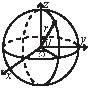
\includegraphics[width=25mm]{content/geometry/sphericalCoordinates}
\end{center}
\[\begin{array}{cc}
x = r\sin\theta\cos\phi & r = \sqrt{x^2+y^2+z^2}\\
y = r\sin\theta\sin\phi & \theta = \textrm{acos}(z/\sqrt{x^2+y^2+z^2})\\
z = r\cos\theta & \phi = \textrm{atan2}(y,x)
\end{array}\]

% \subsection*{Derivatives/Integrals}
% \begin{align*}
% 	\dfrac{d}{dx}\arcsin x = \dfrac{1}{\sqrt{1-x^2}} &&& \dfrac{d}{dx}\arccos x = -\dfrac{1}{\sqrt{1-x^2}} \\
% 	\dfrac{d}{dx}\tan x = 1+\tan^2 x &&& \dfrac{d}{dx}\arctan x = \dfrac{1}{1+x^2} \\
% 	\int\tan ax = -\dfrac{\ln|\cos ax|}{a} &&& \int x\sin ax = \dfrac{\sin ax-ax \cos ax}{a^2} \\
% 	\int e^{-x^2} = \frac{\sqrt \pi}{2} \text{erf}(x) &&& \int xe^{ax}dx = \frac{e^{ax}}{a^2}(ax-1)
% \end{align*}

% Integration by parts:
% \[\int_a^bf(x)g(x)dx = [F(x)g(x)]_a^b-\int_a^bF(x)g'(x)dx\]


% \section{Geometric primitives}
	\kactlimport{Point.h}
	\kactlimport{lineDistance.h}
	\kactlimport{SegmentDistance.h}
	\kactlimport{SegmentIntersection.h}
	\kactlimport{lineIntersection.h}
	\kactlimport{sideOf.h}
	\kactlimport{OnSegment.h}
	\kactlimport{linearTransformation.h}
	% \kactlimport{LineProjectionReflection.h}
	\kactlimport{Angle.h}

% \section{Circles}
	\kactlimport{CircleIntersection.h}
	\kactlimport{CircleTangents.h}
	% \kactlimport{CircleLine.h}
	\kactlimport{CirclePolygonIntersection.h}
	\kactlimport{circumcircle.h}
	\kactlimport{MinimumEnclosingCircle.h}

% \section{Polygons}
	\kactlimport{InsidePolygon.h}
	\kactlimport{PolygonArea.h}
	\kactlimport{PolygonCenter.h}
	\kactlimport{PolygonCut.h}
	% \kactlimport{PolygonUnion.h}
	\kactlimport{ConvexHull.h}
	\kactlimport{HullDiameter.h}
	\kactlimport{PointInsideHull.h}
	\kactlimport{LineHullIntersection.h}

% \section{Misc. Point Set Problems}
	\kactlimport{ClosestPair.h}
	% \kactlimport{ManhattanMST.h}
	\kactlimport{kdTree.h}
	% \kactlimport{DelaunayTriangulation.h}
	\kactlimport{FastDelaunay.h}

% \section{3D}
	\kactlimport{PolyhedronVolume.h}
	\kactlimport{Point3D.h}
	% \kactlimport{3dHull.h}
	% \kactlimport{sphericalDistance.h}
